\section{Methods}
\label{Methods}
% This should be fairly brief, the system is not particularly complex.
For the SORA flights, the MiniPIX was interfaced via USB with Raspberry Pi (RPI) single board computer. Data was collected on the MiniPIX and frame data was sent over serial to the RPI for analysis. During the 2017 flight, only the raw data was stored for post-flight analysis. For the 2018 flight, a custom piece of software was written to concurrently handle analyzing frame data, calculating absorbed dose and handling command and configuration requests from the HASP telemetry interface in addition to storing the raw data. The improvements in the 2018 flight allowed for a near real-time analysis of the radiation environment and the ability to configure the MiniPIX shutter rate and detector parameters via the HASP uplink interface. While being relatively cheap at a price point of 35\$ USD and consuming only \SI{1.2}{\watt} of electrical power, the RPI proved to be robust and operated without glitch for the duration of both flights.


\subsection{Configuration and Calibration}
% Device parameters, threshold, bias voltage, shutter time etc.
The Timepix ASIC consists of 65,536 silicon p-n diodes, each containing its own individual processing circuit. The response of each pixel can never be identical, thus a calibration must be performed for each individual pixel. The appropriate calibration of the MiniPIX detector was applied at The University of Houston following a calibration procedure outlined by Jakubek \cite{mpjakubek}. The source calibration was applied using the 60 keV $^{241}$Am decay line, Sn Fluorescence and $^{55}$Fe gamma rays.
%REVIEW 1 from Renshaw: It would be good to show some result of this calibration, stating that the pixels were all calibrated to have response that is similar within some percentage of the average or even a histogram showing the spread of the calibration.

\subsection{System Design}
% RPI interface to MiniPIX, heatsink design etc.
Additive manufacturing was used to create a custom made case for the MiniPIX device.  The flight assembly is shown in Figure ~\ref{fig:minipix_case} with sindividual components as labeled.  In the early vacuum tests, it was found that the MiniPIX would require a passive cooling method to keep its temperature within operating limits.  At the same time, the ABS plastic enclosure acted as insulation, maintaining the MiniPIX temperature within the operating range.  The MiniPIX was mated to the heatsink via a bracket (not shown in the figure ~\ref{fig:minipix_case}) and with thermal adhesive.
\begin{figure}[H]
    \centering
    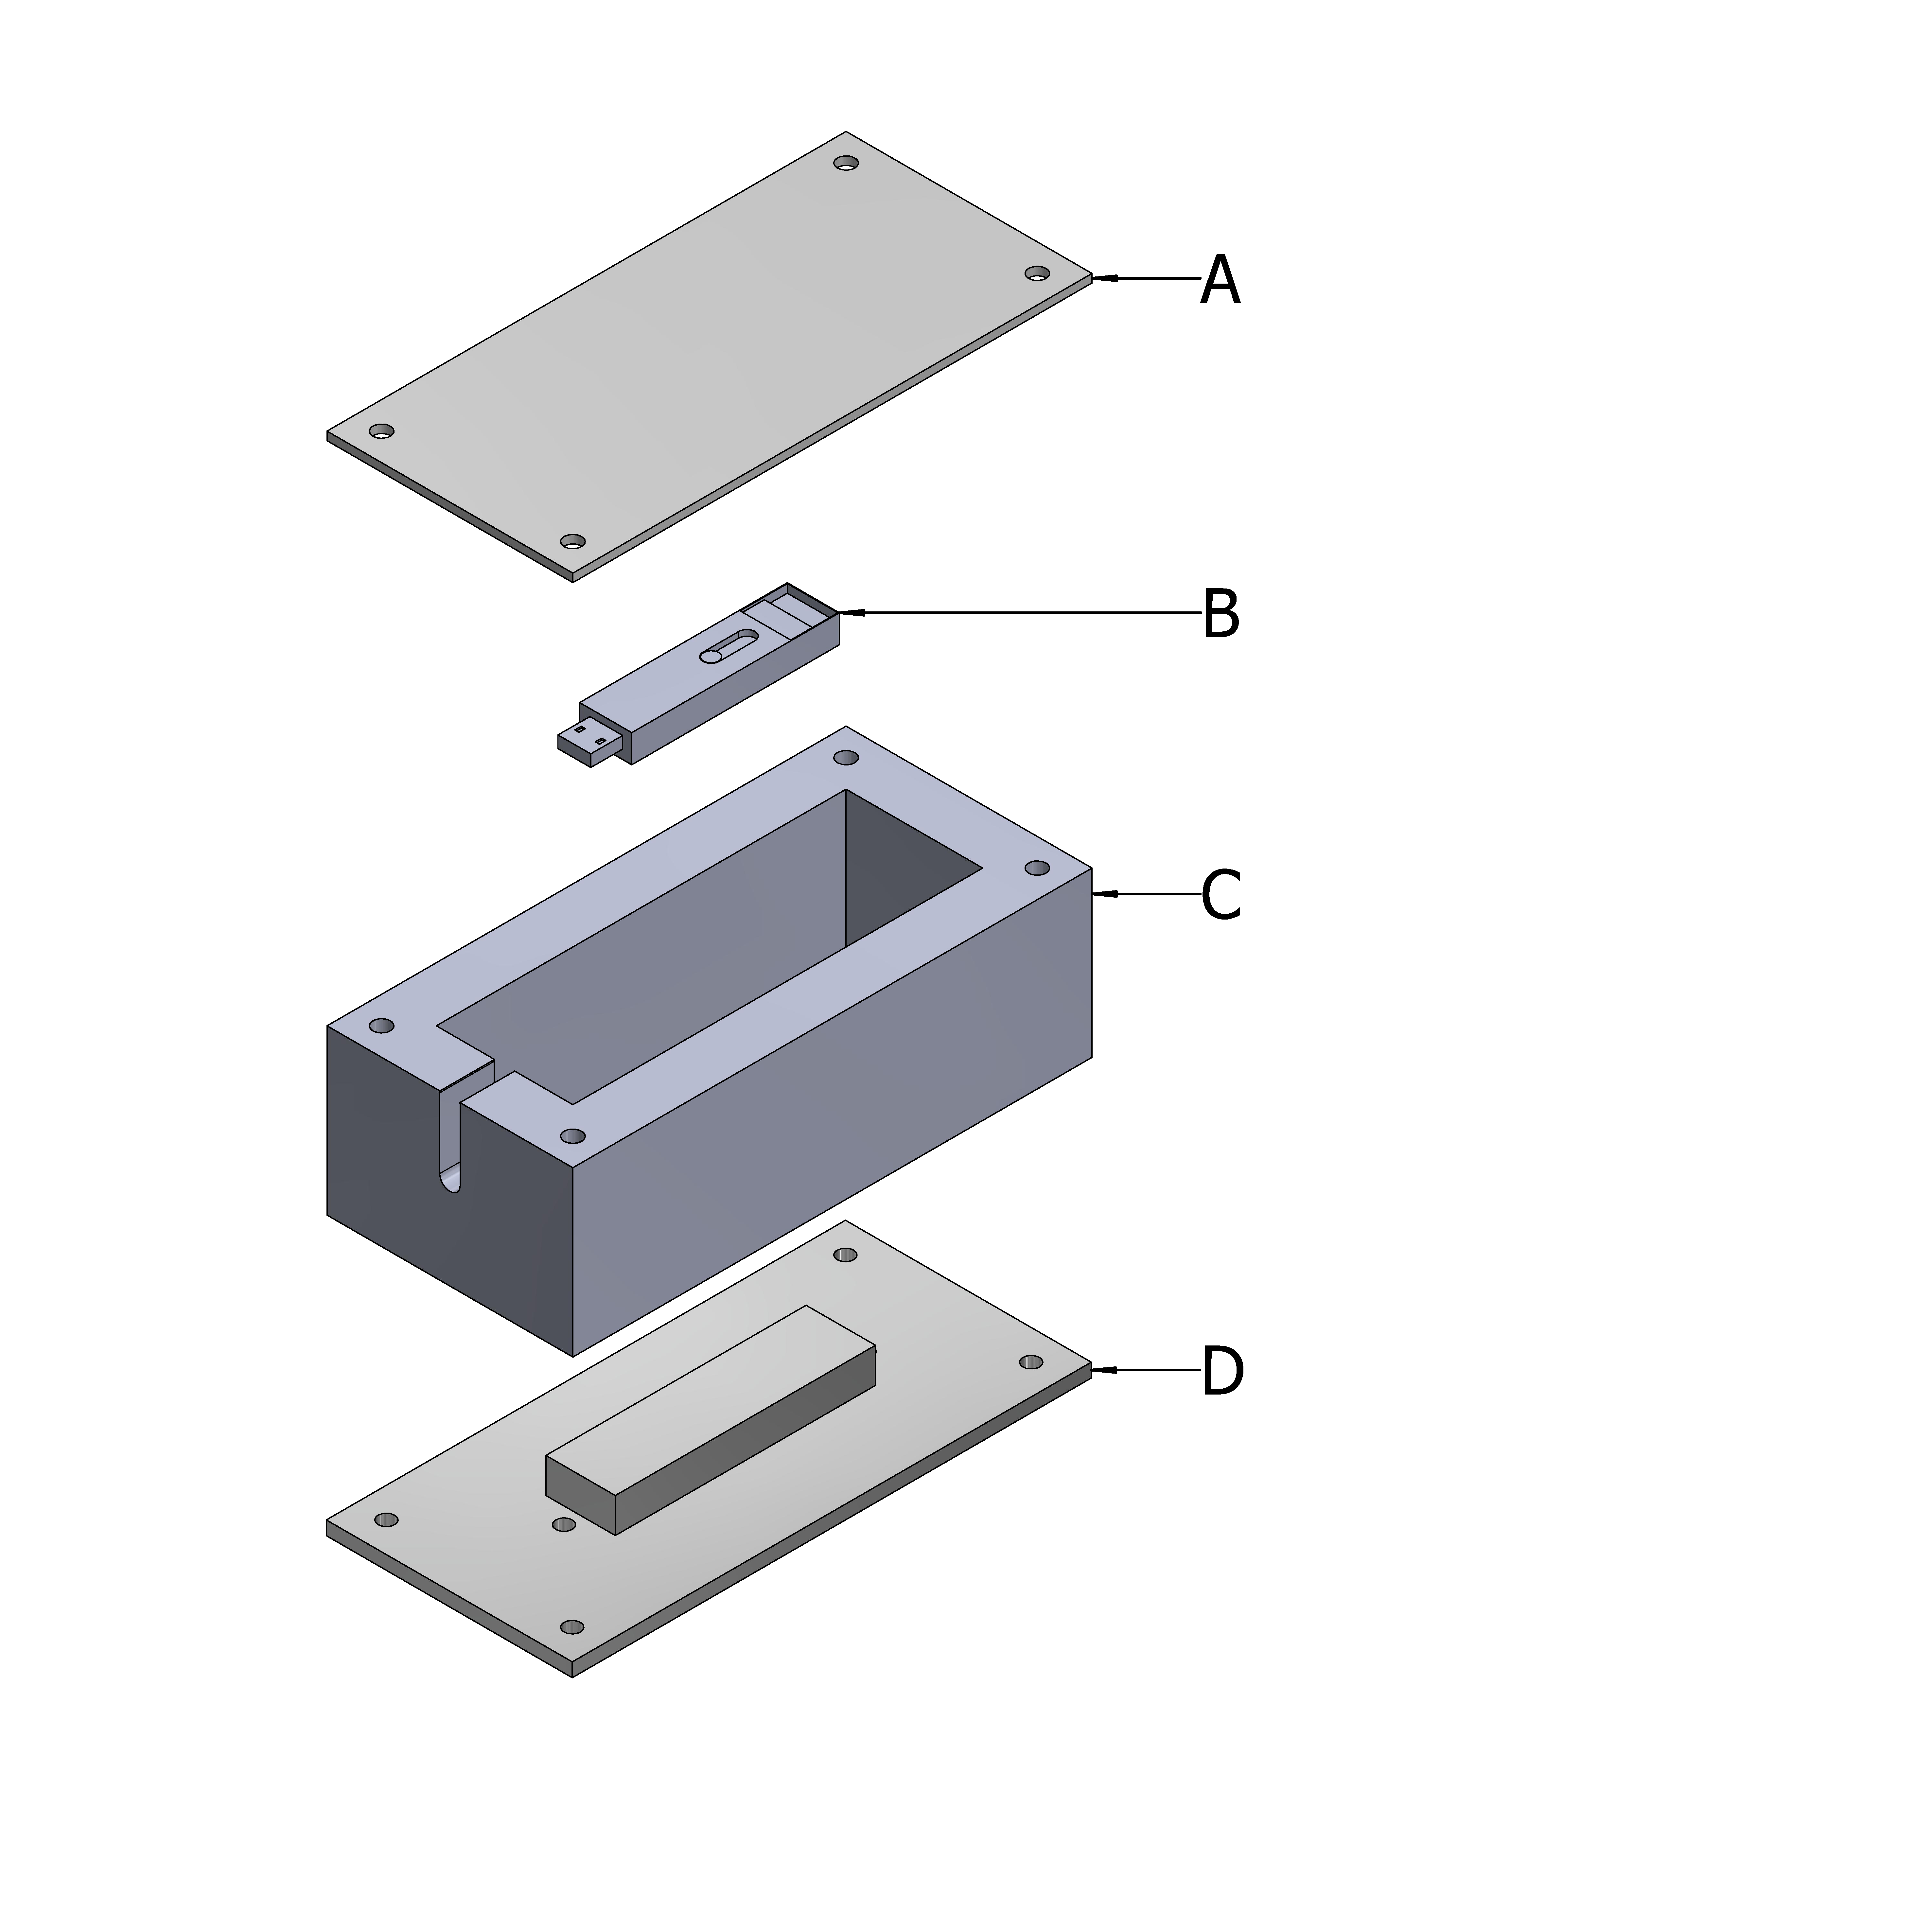
\includegraphics[width=0.45\textwidth]{Minipix_case_assembly.pdf} %from Sam - may need a better image from Steven but this will do for now, it includes all the main parts in a simple way.
%REVIEW 1 from Renshaw: It might be useful to make this a side-by-side figure, with the second figure being a CAD drawing or picture of the payload showing the placement of the RPI and the MiniPIX, along with the other components. 
    %%%Sam: upload new assembly picture
    \caption{MiniPIX~\cite{advacam} Case Assembly. A is the top case assembly, B is the MiniPIX USB device, C is the main case, and D is the heatsink assembly.}
    \label{fig:minipix_case}
\end{figure}
The MiniPIX case allowed for a USB cable to be routed through the enclosure to interface directly to the Raspberry Pi.  This allowed the MiniPIX device to be modular and placed in different configurations for the two flights.  The Raspberry Pi was placed in a separate location within each payload near the power supply.  Overall, each payload was modular and accessible.



